\section{Controlled Verification Methodology}
\textbf{D1 development benchmark.} An Order Platform baseline has five components and five directed relationships. Twenty isolated patches comprise nine no-impact changes, seven violations, and four evolutions. Cases include service bypass, required-edge removal, allow and require-path rules, PostgreSQL aliases, Redis and AMQP additions, a new service, and non-architectural lookalikes. Each declares changed files, graph delta, classification, rule identifiers, and source evidence. Topology intent originated before analyzer integration, but patches and exact evidence lines were refined alongside it. D1 is a co-developed regression oracle, not a blinded holdout.

\textbf{D2 detector corpus.} Five detector groups (HTTP, PostgreSQL, Redis, AMQP publish, and AMQP consume) each contain four positive and four hard-negative source lines: 40 annotated signals in total. Positives exercise aliases, namespaces, environment fallbacks, and supported operations. Negatives include unused imports, custom functions, method-name collisions, comments, and string literals. An annotation binds detector, file, line, expected edge, and source substring. D2 was authored from known v 0.1 weaknesses and guided v 0.2, so the paired result measures targeted regression behavior.

\textbf{Execution and P3 replay.} D1 validates model, manifest, hashes, and patch applicability, then executes an unchanged baseline twice and each individually patched copy twice: 42 analyzer runs. D2 executes each of two pinned analyzer versions twice. P3 creates a fresh Git baseline for every D1 patch, applies it, and runs one cold and one warm diff check. A separate full-head scan provides an equivalence oracle. The same 20 patches are reused, not counted as a third independent dataset. Normalized duplicate outputs exclude timing and cache state. The functional workflow was reproduced on clean Linux and Windows CI runners; latency comes only from the recorded Windows environment.

\begin{figure*}[t]
\centering
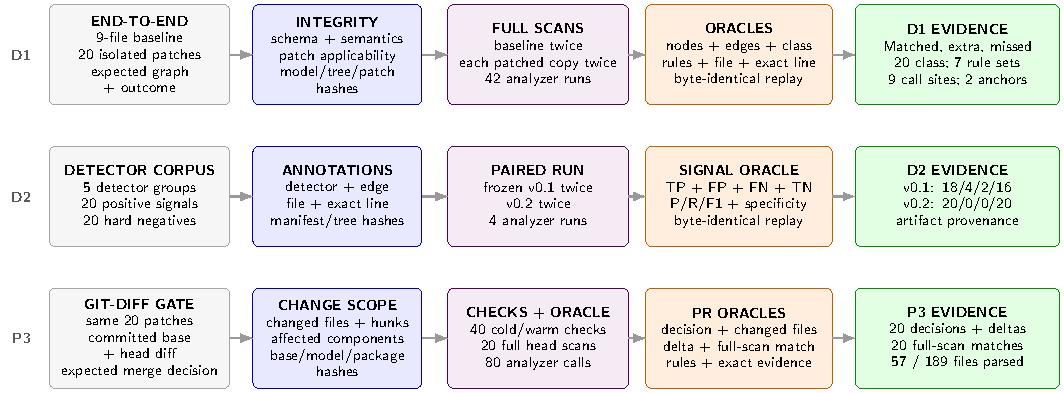
\includegraphics[width=\textwidth]{figures/Fig-2.pdf}
\caption{Controlled verification: full-graph D1 changes, D2 source signals, and incremental P3 replay. All routes use co-developed data.}
\Description{D1 validates isolated patches; D2 checks annotated signals; P3 checks cold and warm Git-diff results against a full scan.}
\label{fig:evaluation-protocol}
\end{figure*}

\textbf{Measures.} D1 reports matched, extra, and missed graph items, separating changed items from repeated baseline structure. Empty changed sets contribute no positive item. Classification uses all 20 cases; rule agreement uses seven violations; evidence agreement splits the original 11 cases post hoc into nine call-site and two missing-relation anchor cases (08 and 17). It requires declared file/line matches per case, not per-finding recall; labels and acceptance rules are unchanged. D2 counts annotated detector signals, not unique edges, with
\[
P=\frac{TP}{TP+FP},\quad R=\frac{TP}{TP+FN},
\]
\[
F_1=\frac{2PR}{P+R},\quad Sp=\frac{TN}{TN+FP}.
\]
Specificity covers only declared hard negatives. P3 checks decision, changed-file and architecture-delta equality, full-scan equivalence, replay, and expected cache miss/hit. Parsed scope is the ratio of affected-component TypeScript file instances to full-head instances. Latency uses nearest-rank $x_{(\lceil pn\rceil)}$ at p50/p95. With 20 samples, p50 is the tenth observation, not the average of the middle pair. Original timings are descriptive, not population or comparative-performance estimates. Node 22.16.0, Windows 10.0.26200, i7-13650HX and 20 logical CPUs were recorded. RAM, power mode, background/thermal load and filesystem-cache state were not recorded.

\textbf{Engineering gates.} The existing protocol required D1 precision/recall at least 0.85, exact decisions/rules/evidence, and deterministic replay; D2 required all annotated positives and negatives correct; P3 required exact replay/full-scan agreement and cache behavior. These are development acceptance rules, not statistical standards. The paper reports counts even where its underlying engineering gate computes rates.

\textbf{Proposed external comparison.} External comparison remains future work; no external-tool comparison was executed within the reported evaluation; no accepted comparator result or common label mapping is available. A module-dependency analyzer is a candidate, but module imports and typed service calls need an explicit, independently reviewed mapping before comparative scoring. The proposed protocol must freeze repositories, versions, configurations, dependency-resolution conditions, and independently authored ground truth before inspecting outputs. Unsupported relations must be separated from misses within common supported scope. The protocol rejects a comparator without a non-empty semantic intersection and requires separately freezing any adapter. A capability discussion cannot complete the baseline or supply an accuracy estimate. Reusing D1 would remain a development-set comparison rather than an independent holdout.
